\documentclass[languages_and_machines.tex]{subfiles}
\begin{document}

\begin{frame}
  \frametitle{Pushdown Automata}

  \begin{block}{Definition}
    \textbf{Non-/Deterministic pushdown automata} := \begin{itemize}
    \item \(S\): a finite set of states
    \item \(A \subseteq S\): a set of accepting states
    \item \(S_0 \in S\): an initial state
    \item \(\Sigma\): a finite alphabet for words
    \item \(\Gamma\): a stack alphabet
    \item \(\Gamma_0\): an initial stack symbol
    \item \(f: S \times \Sigma \times \Gamma \to S \times \Gamma^*\): a transition function
      \pause
    \item \(f: S \times \Sigma \times (\Gamma \cup \{\varepsilon\}) \to S \times \Gamma^*\): a transition function
    \end{itemize}
  \end{block}

  \pause
  Accept by empty stack
\end{frame}

\begin{frame}
  \frametitle{Pushdown Automata}

  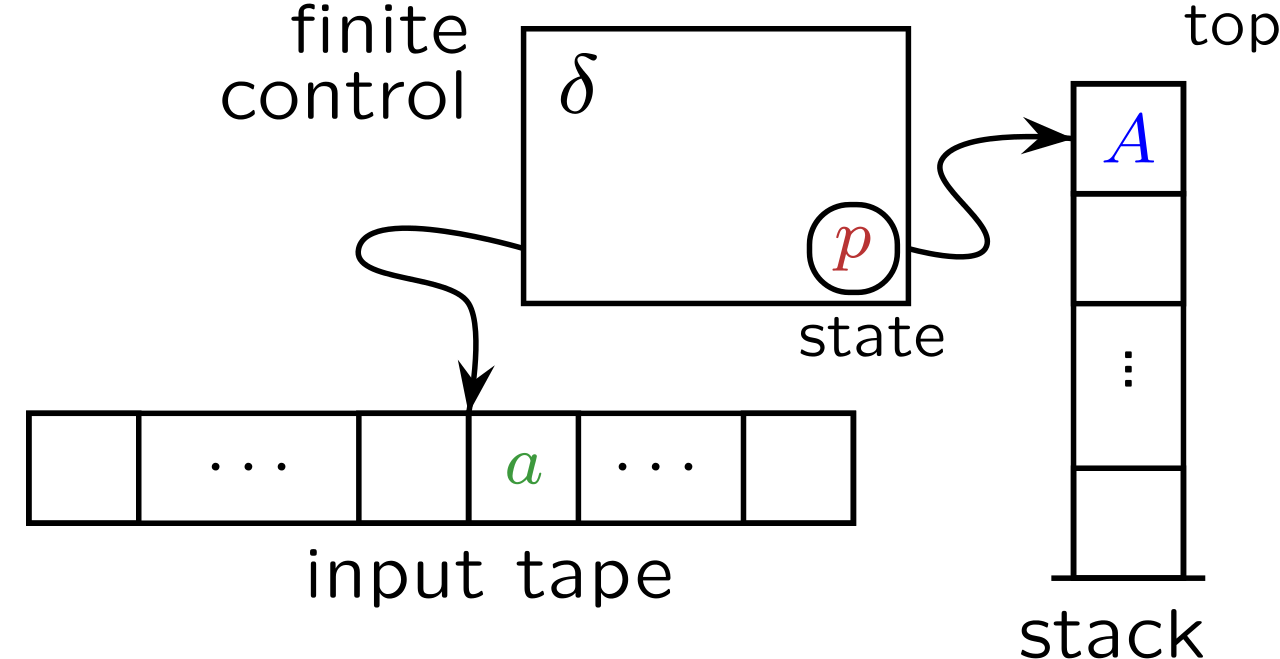
\includegraphics[width=1.0\textwidth]{pushdown_automata.png}
\end{frame}

\begin{frame}
  \frametitle{Pushdown Automata Example}

  \begin{tikzpicture}[->,>=stealth',shorten >=1pt,auto,node distance=4cm,semithick,ampersand replacement=\&]

  \node[initial,state  ] (read)                 {read\only<2>{\!*\!}\only<4>{\!*\!}\only<6>{\!*\!}};
  \node[accepting,state](check) [right of=read] {check\only<8>{\!*\!}\only<10>{\!*\!}\only<12>{\!*\!}};

  \path (read) edge [loop above] node {a, \(x \to x\) a\only<3>{\!*\!}} (read);
  \path (read) edge [loop below] node {b, \(x \to x\) b\only<5>{\!*\!}} (read);
  \path (read) edge [bend left=45] node [above] {\(\varepsilon\), \(x \to x\)\only<7>{\!*\!}} (check);
  \path (read) edge [bend left=-45] node [below] {\(\varepsilon\), \(x \to \varepsilon\)} (check);
  \path (check) edge [loop above] node {a, a \(\to \varepsilon\)\only<11>{\!*\!}} (check);
  \path (check) edge [loop below] node {b, b \(\to \varepsilon\)\only<9>{\!*\!}} (check);
  \end{tikzpicture}

  \pause
  Input: \only<2-3>{\textcolor{red}{a}bba}\only<4-5>{a\textcolor{red}{b}ba}\only<6-7>{abba}\only<8-9>{ab\textcolor{red}{b}a}\only<10-11>{abb\textcolor{red}{a}}\only<12>{abba}

  Stack: H\only<3-11>{a}\only<5-9>{b}

\end{frame}

\begin{comment}
\begin{frame}
  \frametitle{Empty Stack PDA}

  Given PDA with accepting state \(S_f\), PDA with acceptance-by-empty-stack-and-state:
  \pause
  \begin{tikzpicture}[->,>=stealth',shorten >=1pt,auto,node distance=4cm,semithick,ampersand replacement=\&]

  \node[initial  ] (sf)                 {\(S_f\)}
  \node[initial  ] (sfp)                 {\(S_f'\)}

  \path (sf) edge [loop above] node {\(\varepsilon, x \to x\)} (sfp);
  \path (sfp) edge [loop above] node {\(\varepsilon, x \to \varepsilon\)} (sfp);
  \end{tikzpicture}

  Given PDA with acceptance-by-empty-stack-and-state, PDA with acceptence-by-state:
  \pause
  \begin{tikzpicture}[->,>=stealth',shorten >=1pt,auto,node distance=4cm,semithick,ampersand replacement=\&]

  \node[initial  ] (sf)                 {\(S\)}
  \node[initial,accepting  ] (sfp)                 {\(S_f\)}

  \path (sf) edge [loop above] node {\(\varepsilon, \Gamma_0 \to x\)} (sfp);
  \end{tikzpicture}

\end{frame}
\end{comment}

\begin{frame}
  \frametitle{Examples}
  Matched named brackets
  \pause

  State: If left bracket, push bracket-type to stack. If right bracket and correct bracket-type on stack, pop from stack.
\end{frame}

\begin{frame}
  \frametitle{CFG}

  \begin{block}{Definition}
    \textbf{Context-free grammar} := Grammar where all rules are of the form \(A \to \alpha\), where \(\alpha \in (\Sigma \cup \Gamma)^*\).
  \end{block}

  Encodes everything a regular grammar can (repetition, optionals) + ``arbitrary nestedness''

  \begin{itemize}
    \item Matched-brackets
    \pause
      \begin{enumerate}
      \item S \pro [~S~]
      \item S \pro S S
      \item S \pro \emptystr
      \end{enumerate}
    \item \(\{a^nb^n : n \in \mathbb N\}\)
    \pause
      \begin{enumerate}
      \item S \pro aSb
      \item S \pro \emptystr
      \end{enumerate}
    \item Palindromes similar
    \end{itemize}
\end{frame}

\begin{frame}[fragile]
  \frametitle{CFGs in the wild}

  Named brackets

  \pause

\begin{verbatim}
<html>
  <body>
    <h1>This is the tile</h1>
    <p>This is a paragraph.</p>
  </body>
</html>
\end{verbatim}

  \pause

  \href{https://docs.python.org/3/reference/compound_stmts.html}{Programming languages}

  \pause

  95\% of natural languages
\end{frame}

\begin{frame}
  \frametitle{Parse trees}

  \begin{minipage}{0.4\textwidth}
    \begin{enumerate}
    \item S \pro [~S~]
    \item S \pro S S
    \item S \pro \emptystr
    \end{enumerate}

    [[]][]
  \end{minipage}
  \hfill\pause
  \begin{minipage}{0.58\textwidth}
    \begin{forest}
      [S [S [{[}] [S [{[}] [{]}]] [{]}]] [S [{[}] [{]}]]]
    \end{forest}
  \end{minipage}

  \pause
  \vspace{1cm}
  Parse trees for regular languages?
\end{frame}

\begin{frame}
  \frametitle{Ex. Natural language}

  \begin{minipage}{0.42\textwidth}
    \begin{itemize}
    \item S \pro NP VP
    \item NP \pro ADJ N
    \item VP \pro V
    \item VP \pro V NP
    \end{itemize}
  \end{minipage}
  \begin{minipage}{0.54\textwidth}
    \begin{forest}
      for tree={l sep=0.5mm}
      [S [NP [ADJ [the]] [N [fox]]] [VP [V [hit]] [NP [ADJ [the]] [N [ball]]]]]
    \end{forest}
  \end{minipage}

\end{frame}

\begin{frame}
  \frametitle{Ambiguity}

  \begin{block}{Example}
    EXPR \pro EXPR + EXPR \\
    EXPR \pro EXPR * EXPR \\
    EXPR \pro NUMBER
  \end{block}

  \pause

  1 + 3 * 4  

  \pause

  \begin{forest}
    [EXPR [1] [+] [EXPR [3] [*] [4]]]
  \end{forest}\vspace{4mm}
  \begin{forest}
    [EXPR [EXPR [1] [+] [3]] [*] [4]]
  \end{forest}

  Resolution: order rules, \pause order tokens, \pause \textbf{don't}.

\end{frame}

\begin{frame}
  \frametitle{Ambiguity}

  \begin{block}{Example}
    SUM \pro SUM + PROD \\
    SUM \pro PROD \\
    PROD \pro PROD * NUMBER \\
    PROD \pro NUMBER \\
  \end{block}

  \pause

  {\small
  \begin{forest}
    [SUM [1] [+] [PROD [PROD [3]] [*] [4]]]
  \end{forest}
  }

\end{frame}

\begin{frame}
  \frametitle{Ambiguity}

  {\large
    Is a CFG ambiguous?
    \pause
    \alert{Undecidable}
  }

  \vspace{1cm}

  It happens in the wild all the time!


\end{frame}

\begin{frame}
  \frametitle{Ambiguity in natural language}

  British left waffles on Falklands
  
{\small
  \begin{forest}
    [S [NP [ADJ [British]] [N [left]]] [VP [V [waffles]]]]
  \end{forest}
  \begin{forest}
    [S [NP [N [British]]] [VP [V [left]] [NP [N [waffles]]]]]
  \end{forest}
  }

\end{frame}

\begin{frame}
  \frametitle{Ambiguity in natural language}

  ``My parents, Jack and Jill'' refers to 2 or 4 people.

{\small
  \begin{forest}
    for tree={s sep=1mm}
    [LIST [NP [parents]] [{,}] [NP [Jack]] [and] [NP [Jill]]]
  \end{forest}
  \begin{forest}
    [NP [NP [parents]] [APPOS [{,}] [LIST [Jack] [and] [Jill]]]]
  \end{forest}
}

\end{frame}

\begin{frame}
  \frametitle{Ambiguity in natural language}

  ``My father, Jack, and Jill'' refers to 2 or 3 people.

{\small
  \begin{forest}
    for tree={s sep=1mm}
    [LIST [NP [father]] [{,}] [NP [Jack]] [{,}] [and] [NP [Jill]]]
  \end{forest}
  \begin{forest}
    [LIST [NP [father] [APPOS [{,}] [Jack] [{,}]]] [and] [NP [Jill]]]
  \end{forest}
}

\vspace{1cm}
  Lojban

\end{frame}

\begin{frame}[fragile]{}
  \frametitle{Ambiguity in constructed languages}

\begin{verbatim}
class1 obj (class2 ());
\end{verbatim}

{\footnotesize
\pause
  \begin{forest}
    for tree={s sep=0.5mm}
    [STMT [OBJ-DECL [TYPE] [NAME] [(] [ARGS [EXPR [CALLABLE] [(] [)]]] [)]]]
  \end{forest}
\pause
  \begin{forest}
    for tree={s sep=0.5mm}
    [STMT [FN-PTR [TYPE] [NAME] [(] [ARGS [FN-PTR [TYPE] [(] [)]]] [)]]]
  \end{forest}
}


\end{frame}

\begin{frame}[fragile]
  \frametitle{Public Service Announcement}

\begin{verbatim}
// class1 constructed from class2
class1 obj ((class2 ()));
class1 obj {class2 {}}; // C++11

// Function pointer
class1 obj (class2 name ());
\end{verbatim}

\end{frame}

\begin{comment}
\begin{frame}
  \frametitle{CFG \(\iff\) PDA}

  CFG can generate all strings accepted by PDA.

  \pause

  Given PDA with acceptance-by-empty-stack, suppose \(f(\textcolor{red}{s_{\mathrm{top}}, S, x_{n}}) = (\textcolor{green}{S', s_{\mathrm{top}}'})\).

  Complete-state

  \pause

  \(s_0 s_1 \dotsb \textcolor{red}{s_{\mathrm{top}} S x_{n}} x_{n-1} \dotsb x_{\mathrm{end}}\)

  \pause

  \(s_0 s_1 \dotsb \textcolor{green}{s_{\mathrm{top}}' S'} x_{n-1} \dotsb x_{\mathrm{end}}\)

  \pause

  Rule: \(\textcolor{green}{s_{\mathrm{top}}' S'} \to \textcolor{red}{s_{\mathrm{top}} S x_{n}}\)

  Run the PDA backwards.

\end{frame}

\begin{frame}
  \frametitle{CFG \(\iff\) PDA}

  \begin{enumerate}
  \item Start symbol is the complete-state with empty stack and accepting state \(S \to \Gamma_0 S_f\).
    \pause
  \item Allow the stack to grow arbitrarily \(\Gamma_0 \to \Gamma_0 \Gamma_i\), so we have a stack \(\Gamma_0 \Gamma_i \dotsb S_f\).
    \pause
  \item Do some \(s_{\mathrm{top}} S} \to s_{\mathrm{top}} S x_{n}\), so we have \(\Gamma_0 \Gamma_i \dotsb S_f x_{j} x_{j+1} \dotsb x_{n}\)
    \pause
  \item Erase the stack and state \(\Gamma_0 \Gamma_i \to \varepsilon\), so we have a stack \(\Gamma_0 \Gamma_i \dotsb S_f\).
  \end{enumerate}
  % Several of these are non-context free rules

\end{frame}
\end{comment}

\begin{comment}
\begin{frame}
  \frametitle{Top-down parsing}

  \(\sigma(S, q_1, \varepsilon) = \{(\alpha, q_1)\}\) when \(S \to \alpha\)

  \(\sigma(a, q_1, a) = \{(\varepsilon, q_1)\}\) for all \(a\) \\

  \(S \to (~S~)\)

  \(S \to SS\)

  \(S \to \varepsilon\) \\
v
  Stack: \only<1>{S}\only<2>{SS}\only<3>{S(S)}\only<4>{S(S}\only<5>{S(}\only<6>{S}\only<7>{(S)}\only<8>{(S}\only<9>{(()}\only<10>{((}\only<11>{(}\only<12>{}

  Input: \only<1-2>{(())()}\only<3>{(())()}\only<4-5>{(())(}\only<6-7>{(())}\only<8-9>{(()}\only<10>{((}\only<11>{(}\only<12>{}

\end{frame}
\end{comment}

\begin{frame}
  \frametitle{Bottom-up parsing}

  % \(\sigma(\alpha, q_1, \varepsilon) = \{(S, q_1)\}\) ``reduce'' when \(S \to \alpha\)

  % \(\sigma(\alpha, q_1, a) = \{(\alpha a, q_1)\}\) ``shift'' for all \(\alpha\) and \(a\)

  \(S \to (~S~)\)

  \(S \to \varepsilon\)

  Stack: \only<1>{}\only<2>{(}\only<3>{((}\only<4>{((S}\only<5>{((S)}\only<6>{(S}\only<7>{(S)}\only<8>{S}\only<9>{S(}\only<10>{S(S}\only<11>{S(S)}\only<12>{SS}\only<13>{S}

  Input: \only<1>{(())()}\only<2>{())()}\only<3-4>{))()}\only<5-6>{)()}\only<7-8>{()}\only<9-10>{)}\only<11>{}

\end{frame}

\begin{comment}
\begin{frame}
  \frametitle{Parsing algorithms}

  \begin{block}{Example}
    SUM \pro PROD \\
    SUM \pro SUM + PROD \\
    PROD \pro NUMBER \\
    PROD \pro PROD * NUMBER \\
  \end{block}

  Input: 1 + 3 * 4

  SUM \pro \only<2>{PROD \pro NUMBER}\only<3>{\sout{PROD}}\only<4->{SUM + PROD \pro \(\dotsb\)}

  \only<5->{SUM \pro}\only<6>{?}\only<7>{\textit{Peak at ``1 + ''}}\only<8->{SUM + PROD \pro \(\dotsb\)}

  \only<9->{Compiler compilers

    \begin{itemize}
    \item LALR(k) (1973)
    \item LL(*) (1969)
    \end{itemize}
  }

\end{frame}
\end{comment}

\begin{frame}
  \frametitle{Properties of CFL}

  \begin{itemize}
  \item Closed under disjunction (prove using PDAs) \pause \emptystr transitions to start state of machine 1 OR 2.
    \pause
  \item Closed under Kleene-* (prove using empty-stack PDAs) \pause \emptystr transition from accepting state to start state.
    \pause
  \item Closed under conjunction \pause NOT
    \pause
  \item Chomsky Normal Form (\(A \to BC\), \(A \to a\), exception for \(\varepsilon \in L\)) (\href{https://en.wikipedia.org/wiki/Chomsky_normal_form\#Converting_a_grammar_to_Chomsky_normal_form}{algorithm} 1959)
    \pause
  \item Chomsky--Sch\"utzenberger Theorem (1963): CFG = named-bracket \(\cap\) regular
    % \begin{itemize} 
    % \item \(\{a^n b^n : n \in \mathbb N\} = \{\textrm{nested pairs of a and b \} \cup \{a^i b^k : i, k \in \mathbb N\}\)
    % \end{itemize}
  \end{itemize}
\end{frame}

\begin{frame}
  \frametitle{Pumping lemma for CFG}

  \begin{minipage}{0.3\textwidth}
    \small
    For all \(s \in L\) and \(\lvert s \rvert \geq n\),
    \begin{itemize}
    \item \(s = uvwxy\)
    \item \(uv^i w x^i y \in L\)
    \item \(\lvert vx \rvert \geq 1\) 
    \item \(\lvert vwx \rvert \leq p\).
    \end{itemize}
  \end{minipage}
  \hfill\pause
  \begin{minipage}{0.68\textwidth}
    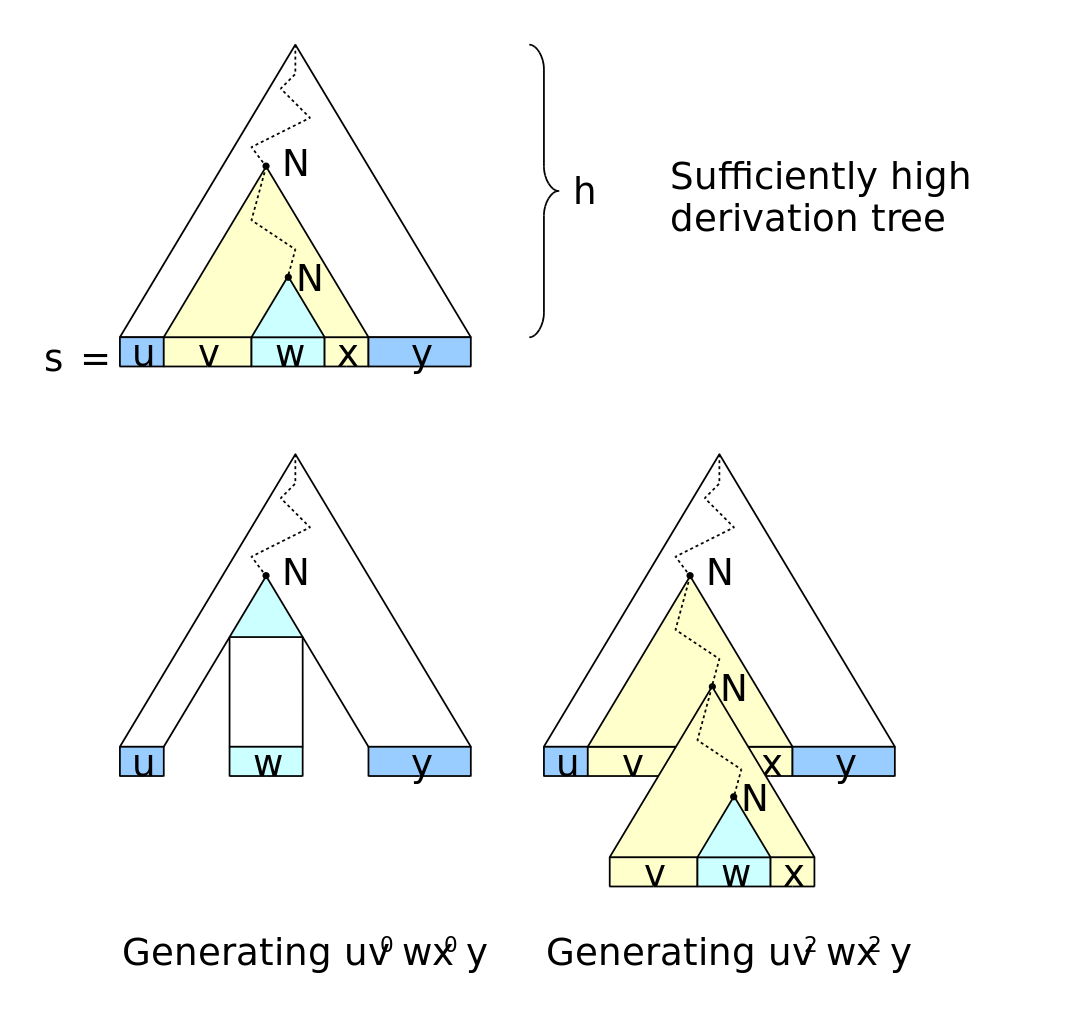
\includegraphics[width=\textwidth]{pumping_lemma_for_cfg.png}

    {\tiny Figure from \href{https://commons.wikimedia.org/wiki/File:Pumping_lemma_for_context-free_languages.svg}{WikiMedia}}
  \end{minipage}
\end{frame}

\begin{frame}
  \frametitle{Harder languages}

  \begin{itemize}
  \item \(\{a^n b^n c^n : n \in \mathbb N\}\). No `pumpable' substrings within \(n\).
    \begin{itemize}
      \pause
    \item Note that \(\{a^n b^n c^n\} = \{a^n b^n c^k\} \cup \{a^n b^k c^k\}\) \(\implies\) CFLs \textbf{are not closed} under conjunction.
    \item But they \textbf{are closed} under disjunction, so they \textbf{are not closed} under complementation.
    \end{itemize}
    \pause
  \item \(\{w^2 : w \in \Sigma^*\}\) (``stutters'')
    \pause
  \item Challenge: prove \(x : n_a(x) = k n_b(x)\) is not a CFL where \(n_a(x)\) is the number of ``a'' in \(x\).
    \pause
  \item Swiss-German cross-serial dependencies \(\mathrm{adj}_1~\mathrm{adj}_2\dotsb \mathrm{adj}_n~\mathrm{noun}_1~\mathrm{noun}_2 \dotsb \mathrm{noun}_n\)
    \pause
  \item Programming language with no undefined terms
  \end{itemize}
\end{frame}

\end{document}

%%% Local Variables:
%%% mode: latex
%%% TeX-master: t
%%% End:
